\documentclass[11pt]{article}

\usepackage[T1]{fontenc}
\usepackage{amsmath,amssymb,amsthm,mathtools}
\usepackage{newtxtext,newtxmath}
\usepackage[margin=1.05in]{geometry}
\usepackage{booktabs}
\usepackage{enumitem}
\usepackage{graphicx}
\usepackage{microtype}
\usepackage{xcolor}
\usepackage[hidelinks]{hyperref}
\usepackage[nameinlink,noabbrev]{cleveref}

\hypersetup{
  pdftitle={Energy and Backreaction Bounds for Finite-Pointer Observer
  Entropy},
  pdfauthor={Brian Fioca},
  pdfsubject={Localized thermal dephasing, finite-pointer Renyi entropy, and
  observer-code accuracy in a de Sitter static patch}
}

\newtheorem{theorem}{Theorem}[section]
\newtheorem{lemma}[theorem]{Lemma}
\newtheorem{proposition}[theorem]{Proposition}
\newtheorem{corollary}[theorem]{Corollary}
\theoremstyle{definition}
\newtheorem{definition}[theorem]{Definition}
\theoremstyle{remark}
\newtheorem{remark}[theorem]{Remark}

\newcommand{\R}{\mathbb R}
\newcommand{\cD}{\mathcal D}
\newcommand{\cE}{\mathcal E}
\newcommand{\cH}{\mathcal H}
\newcommand{\dd}{\,\mathrm d}
\newcommand{\eobs}{\epsilon_{\mathrm{obs}}}
\newcommand{\EK}{E_{K}}
\newcommand{\Ebar}{\overline E_{K}}
\newcommand{\Pcl}{P_{\rm cl}}
\newcommand{\Tr}{\operatorname{Tr}}
\newcommand{\supp}{\operatorname{supp}}
\newcommand{\sech}{\operatorname{sech}}
\newcommand{\norm}[1]{\left\lVert#1\right\rVert}
\newcommand{\abs}[1]{\left\lvert#1\right\rvert}
\newcommand{\ip}[2]{\left\langle#1,#2\right\rangle}
\newcommand{\ket}[1]{\left\lvert#1\right\rangle}
\newcommand{\bra}[1]{\left\langle#1\right\rvert}

\title{Energy and Backreaction Bounds\\
for Finite-Pointer Observer Entropy}
\author{Brian Fioca}
\date{Draft of June 2026}

\begin{document}
\maketitle

\begin{abstract}
The observer rule of Harlow, Usatyuk, and Zhao is controlled by a second
R\'enyi entropy, but does not derive the field resources needed to produce its
pointer-basis record.  We give such a bound in an exactly solvable local
field model.  A finite pointer controls compact sources for a free scalar,
producing a Schur dephasing channel with conditional final data $p_i$.  If
$w_i$ are the pointer weights,
$\Pcl=\sum_iw_i^2$, and
$\Ebar=\sum_iw_i\norm{p_i-\bar p}^2/2$, then final support in $[0,L]$ implies
\[
 \Tr\rho_P^2\geq\Pcl+(1-\Pcl)
 \exp\!\left[-\frac{\mathcal C_\beta(L)\Ebar}{1-\Pcl}\right],
 \qquad
 S_2(\rho_P)\leq\min\{H_2(w),\mathcal C_\beta(L)\Ebar\}.
\]
The coefficient is exact:
$\mathcal C_\beta(L)=2L\Lambda(\pi L/\beta)$, where $\Lambda(\tau)$ is the
simple top eigenvalue of the positive compact
kernel
$\pi^{-1}\log[\sinh(\tau(u+v))/\sinh(\tau|u-v|)]$ on $(0,1)$.
The entropy bound is saturated in the symmetric binary top-mode sector; no
general-$d$ sharpness is claimed.  For
the conformally coupled massless scalar in a four-dimensional de Sitter static
patch, $\beta=2\pi R$, the same coefficient controls all angular and canonical
sectors, with $\mathcal C_{2\pi R}(L)=RC_{\rm opt}(L/R)$.

Using a purified field record as the nonideal observer record in the simple
Harlow--Usatyuk--Zhao random code, the Haar-averaged squared inner-product
fluctuation for an orthogonal CRT-real matter pair is therefore bounded below
by the displayed physical purity, up to the exact finite-code factor
$D/(D+2)$.  Finally, if every conditional spherical $q_i=0$ branch obeys a
local final-slice constraint budget $Q_{b,i}\leq\delta$, then
\[
 S_2(\rho_P)\leq
 \delta\frac{R^2}{G}\,
 \frac{C_{\rm opt}(y)\tanh y\,\sech^2y}{2}.
\]
This is a fixed-background channel plus a branchwise final-slice constraint
corollary, not a coupled gravity theorem.  The prescribed pointer and source
exclude actuator work, autonomous-observer stress, and a deterministic error
floor for every fixed code.
\end{abstract}

\section{Introduction}
\label{sec:introduction}

A localized quantum reference or observer is not only an abstract register.
It must couple to fields for a finite time and within a finite region, and the
resulting field state carries energy and stress.  This elementary observation
is often hidden when an ideal observer is represented directly by a dephasing
map.  Our purpose is to quantify it in one continuum model where the channel,
the field stress, and the causal support can all be treated without a weak
coupling expansion.

Harlow, Usatyuk, and Zhao motivate an ideal observer by a quantum-to-classical
channel that removes off-diagonal blocks in a stable pointer
basis~\cite{HarlowUsatyukZhao2025}.  We use complete pointer dephasing as that
operational target.  Our channel distance below is not their gravitational
encoding error, and the qubit in this model is not identified with their
observer entropy $S_{\rm Ob}$.

Gapless two-level detectors linearly coupled to free fields provide exactly
such a model.  Their time-ordered evolution is an exact Weyl displacement,
because free-field commutators are c-numbers.  Landulfo used this fact for
relativistic communication channels~\cite{Landulfo2016}; Barcellos and Landulfo
derived the corresponding field-energy and switching-work
accounting~\cite{BarcellosLandulfo2021}.  More recently, this solvable detector
has been used for a nonperturbative treatment of
Danielson--Satishchandran--Wald (DSW) decoherence~\cite{BatistaEtAl2026}.
Killing-horizon decoherence itself, its local two-point-function formulation,
and its de Sitter specialization are by now well
developed~\cite{DSW2023,GrallaWei2024,DSW2025,Li2025}.

Those results determine the dephasing functional for a chosen source.  They do
not by themselves eliminate the source and ask how large that functional can
be at fixed post-switch field energy and finite causal support.  This is the
question addressed here.  In the conformal scalar static-patch model, the
answer reduces to a localized comparison between negative powers of the
one-particle Hamiltonian and the energy norm.  The low-frequency thermal
enhancement is dangerous globally, but compact support turns the relevant
compressed inverse operators into bounded forms.

Let $R$ be the de Sitter radius, let a smooth source be supported inside a
centered areal ball of radius $a<R$ for a static-time interval of length $T$,
and let $\eobs$ denote the halved diamond distance between the resulting
pointer channel and complete pointer dephasing.  Our main result is
\begin{equation}
 \log\frac{1}{2\eobs}
 \leq \EK R C_{\rm opt}(y)
 \leq \EK R F(y),
 \qquad
 y=\operatorname{arctanh}(a/R)+T/R,
 \label{eq:main-intro}
\end{equation}
where
\begin{equation}
 C_{\rm opt}(y)=2y\Lambda(y/2),
 \qquad
 F(y)=\frac{4\operatorname{arsinh}(1)}{\pi}y
      +\frac{8}{\pi^3}y^2 .
 \label{eq:cost-intro}
\end{equation}
Here $\Lambda(\tau)$ is the top eigenvalue of the explicit positive compact
kernel
\begin{equation}
 k_\tau(u,v)=\frac1\pi
 \log\frac{\sinh[\tau(u+v)]}{\sinh[\tau\abs{u-v}]}
 \quad\hbox{on }L^2(0,1).
 \label{eq:kernel-intro}
\end{equation}
The field energy $\EK$ is generated by the same source that defines the
channel.  No detector coupling remains in \cref{eq:main-intro}.  The estimate
holds for the full conformal scalar, not only its spherical sector.  The
exact optimizer is the unique positive top eigenfunction of
\cref{eq:kernel-intro} in the s-wave momentum sector.  A resolvent expansion
shows that the angular potential improves the complete thermal kernel, while
explicit momentum lower bounds dominate the field-coordinate sector for every
$y>0$.

Largest-eigenvalue and isoperimetric questions for Riesz-potential operators
have an established spectral literature, including spherical and hyperbolic
geometries~\cite{RuzhanskySuragan2016}.  We do not claim novelty for the
compact-operator variational principle or its Perron--Frobenius conclusion.
The candidate contribution is the exact reflected KMS kernel selected by the
detector problem, the reduction of all angular and canonical sectors to that
one operator, and the resulting operational support asymptotics.

The exact coefficient has controlled support asymptotics.  Globally,
\begin{equation}
 \max\left\{\frac{3y}{\pi},\frac{8y^2}{\pi^3}\right\}
 \leq C_{\rm opt}(y)
 \leq F(y).
 \label{eq:two-sided-intro}
\end{equation}
The ratio between the analytic upper and lower linear coefficients is
$4\operatorname{arsinh}(1)/3\simeq1.17516$.  More sharply,
$C_{\rm opt}(y)-2y\Lambda(0)=O(y^3)$ with a rigorous remainder
$y^3/(6\pi)$, and
$C_{\rm opt}(y)=8y^2/\pi^3+O(1)$.  Thus the linear small-support law and the
quadratic large-support law are both intrinsic rather than artifacts of the
original one-sided estimate.

The relation to gravity is deliberately limited but exact.  In the spherical
subclass one may finish with vanishing field coordinate and nonzero field
momentum.  The momentum density then vanishes.  The optical Killing-energy
measure is exactly the mass measure in the Einstein--scalar Hamiltonian
constraint with vanishing extrinsic curvature, giving a necessary radial
metric cost and an explicit nonempty local weak-constraint window.  The
nonzero scalar momentum means the full matter data are not time-reflection
symmetric.  This is a theorem about initial data on the final post-switch
slice, not a derivation of the detector channel on its own perturbed geometry.

There is also a close conceptual comparison with Bekenstein-type bounds.
Hollands, Longo, and Morsella recently proved a model-independent
local-entropy bound for localized Klein--Gordon wave packets
\cite{HollandsLongoMorsella2026}.  Their modular entropy and our pointer
dephasing exponent are different quadratic forms.  We give two radial packet
sequences showing that neither uniformly bounds the other at fixed radius.
Thus \cref{eq:main-intro} should be read as an operational dephasing analogue,
not as the first localization--information--energy inequality in QFT.

The paper is organized as follows.  \Cref{sec:model} fixes the static-patch
model and recalls the exact channel and stress identities.  \Cref{sec:bound}
proves the sharp all-angular localization--energy theorem.
\Cref{sec:construction} gives explicit trial profiles and smooth source
realization.
\Cref{sec:gravity} constructs the final Einstein--scalar constraint data.
\Cref{sec:comparison} compares the result with local entropy and horizon
decoherence.  \Cref{sec:discussion} states the claim boundary and open
problems.

\section{Static-patch model and exact pointer channel}
\label{sec:model}

\subsection{Optical partial waves}

In static coordinates, four-dimensional de Sitter space has
\begin{equation}
 \dd s^2=-N(r)\dd t^2+\frac{\dd r^2}{N(r)}+r^2\dd\Omega_2^2,
 \qquad N(r)=1-\frac{r^2}{R^2},
 \qquad 0\leq r<R .
 \label{eq:static-metric}
\end{equation}
Introduce the optical radius
\begin{equation}
 x=R\operatorname{arctanh}(r/R),
 \qquad r=R\tanh(x/R),
 \qquad \Omega(x)=\sech(x/R).
 \label{eq:optical-radius}
\end{equation}
Then $g_{\rm dS}=\Omega^2g_{\rm opt}$, where
\begin{equation}
 g_{\rm opt}=-\dd t^2+\dd x^2+R^2\sinh^2(x/R)\dd\Omega_2^2 .
\end{equation}
For the conformally coupled massless scalar, spherical-harmonic decomposition
and the standard radial rescaling give the positive operators
\begin{equation}
 A_\ell=-\frac{\dd^2}{\dd x^2}
 +\frac{\ell(\ell+1)}{R^2\sinh^2(x/R)},
 \qquad h_\ell=A_\ell^{1/2}
 \label{eq:partial-wave-hamiltonian}
\end{equation}
on $L^2(\R_+)$, with the regular Dirichlet condition at $x=0$.
The Bunch--Davies state restricted to the static patch is KMS at
\begin{equation}
 \beta=2\pi R
 \label{eq:beta}
\end{equation}
for the static Killing flow.  We use this standard identification throughout.

Let $(q_{\ell m},p_{\ell m})$ denote real final Cauchy data for the rescaled
partial waves.  For smooth compact data, the thermal quadratic form and the
Killing energy are
\begin{align}
 \Gamma_{\ell m}
 &=\ip{q_{\ell m}}{h_\ell\coth(\beta h_\ell/2)q_{\ell m}}
   +\ip{p_{\ell m}}{h_\ell^{-1}\coth(\beta h_\ell/2)p_{\ell m}},
 \label{eq:gamma-sector}\\
 E_{\ell m}
 &=\frac12\left(\norm{h_\ell q_{\ell m}}^2
                    +\norm{p_{\ell m}}^2\right).
 \label{eq:energy-sector}
\end{align}
We write $\Gamma=\sum_{\ell m}\Gamma_{\ell m}$ and
$\EK=\sum_{\ell m}E_{\ell m}$.  Smooth angular data make these sums finite in
the needed form domains.

For $\ell=0$, the unitary sine transform diagonalizes $h_0$.  With hats
denoting that transform,
\begin{align}
 \Gamma_{00}
 &=\int_0^\infty\coth(\beta k/2)
 \left(k\abs{\widehat q(k)}^2+\frac{\abs{\widehat p(k)}^2}{k}\right)\dd k,
 \label{eq:gamma-sine}\\
 E_{00}
 &=\frac12\int_0^\infty
 \left(k^2\abs{\widehat q(k)}^2+\abs{\widehat p(k)}^2\right)\dd k.
 \label{eq:energy-sine}
\end{align}

\subsection{Local interaction and exact channel}

Let $P$ be a degenerate pointer qubit with pointer observable $Z_P$.  We
couple it to the physical scalar by
\begin{equation}
 S_{\rm int}=-\int_{\mathcal M}\sqrt{-g}\,J(X)\phi(X)Z_P\dd^4X,
 \qquad J\in C_c^\infty(\mathcal M;\R).
 \label{eq:interaction}
\end{equation}
The switching function and spatial smearing are both included in $J$.  Since
the commutator of two smeared free fields is a c-number, every Magnus term
beyond second order vanishes.  Up to a source-dependent scalar phase,
\begin{equation}
 U_J=e^{i\Xi[J]}e^{-i\phi(J)Z_P}.
 \label{eq:exact-unitary}
\end{equation}
This standard exact evolution is reviewed in
\cite{Landulfo2016,BarcellosLandulfo2021,BatistaEtAl2026}.
The interaction is compactly supported, and its densities commute at
spacelike separation because $Z_P$ is fixed and the scalar field is
microcausal.  Nevertheless, the same finite-dimensional operator $Z_P$
appears across the smearing.  Generic spatially extended nonrelativistic
detectors can violate causal factorization~\cite{deRamonEtAl2021}; fully
relativistic localized probe fields provide a systematic replacement
framework~\cite{PercheEtAl2024}.  We therefore treat
\cref{eq:interaction} as the standard prescribed gapless-detector
idealization, not as an autonomous pointer field or material actuator.

Let $E$ denote the causal propagator and $K$ the positive-frequency map for the
static one-particle structure.  Tracing the Bunch--Davies field state gives a
pointer dephasing channel
\begin{equation}
 \cD_\kappa
 \begin{pmatrix}a&b\\c&d\end{pmatrix}
 =\begin{pmatrix}a&\kappa b\\\overline\kappa c&d\end{pmatrix},
 \qquad
 \abs\kappa=e^{-\Gamma},
 \qquad
 \Gamma=2\ip{KEJ}{\coth(\beta h/2)KEJ}.
 \label{eq:dephasing-channel}
\end{equation}
The phase of $\kappa$ is a pointer rotation and is irrelevant to the distance
from complete dephasing.  If $\cD_0$ denotes complete dephasing, then
\begin{equation}
 \eobs:=\frac12\norm{\cD_\kappa-\cD_0}_\diamond
 =\frac12\abs\kappa=\frac12e^{-\Gamma}.
 \label{eq:diamond-error}
\end{equation}
The equality follows from
$\cD_\kappa-\cD_0=(\kappa/2)(\mathrm{id}-\operatorname{Ad}_{Z_P})$ after the
correctable phase is removed, and it is saturated by a pointer superposition.
The target $\cD_0$ is the binary instance of the quantum-to-classical pointer
channel used in the observer rule of Harlow, Usatyuk, and
Zhao~\cite{HarlowUsatyukZhao2025}.  The error $\eobs$ measures this channel
approximation only; it is not their closed-universe encoding error and is not
identified with $e^{-S_{\rm Ob}}$.

After the source switches off, the two conditional field states are opposite
coherent displacements.  Their common excess Killing energy and excess
renormalized stress are
\begin{equation}
 \EK=\ip{KEJ}{hKEJ},
 \qquad
 \Delta\langle T_{ab}^{\rm ren}\rangle=T_{ab}[\phi_J].
 \label{eq:energy-stress}
\end{equation}
The state-independent Hadamard subtraction cancels in the difference, and the
background one-point function vanishes.  Equation~\eqref{eq:energy-stress}
prices the post-switch scalar field generated by \emph{the same} $J$ as the
channel.  It does not include the stress of a clock, trap, or material device
that realizes the prescribed coupling.

\subsection{Causal support}

Suppose $J$ is supported inside the centered areal ball $r\leq a<R$ during a
static-time interval of length $T$.  Its optical radius is
\begin{equation}
 \ell=R\operatorname{arctanh}(a/R).
 \label{eq:source-optical-radius}
\end{equation}
Finite propagation in the optical metric implies that the final Cauchy data of
every partial wave are supported in
\begin{equation}
 0\leq x\leq L,
 \qquad L=\ell+T.
 \label{eq:causal-support}
\end{equation}
No spectral cutoff or hard spatial wall is introduced.

\section{Sharp final-support thermal bounds}
\label{sec:bound}

Let $P_L$ be multiplication by $(0,L)$ on $L^2(\R_+)$.  We first solve the
momentum problem at arbitrary inverse temperature $\beta$.  We then impose the
de Sitter relation $\beta=2\pi R$ and prove that the same momentum sector is
the optimum over every angular and canonical sector.

\begin{lemma}[Compressed half-line inverses]
\label{lem:compressed-inverses}
For $h_0=\sqrt{-\partial_x^2}$ with the half-line Dirichlet condition,
\begin{align}
 (P_Lh_0^{-1}P_L)(x,y)
 &=\frac1\pi\log\frac{x+y}{\abs{x-y}},
 \label{eq:hminusone-kernel}\\
 (P_Lh_0^{-2}P_L)(x,y)
 &=\min(x,y).
 \label{eq:hminustwo-kernel}
\end{align}
Moreover,
\begin{align}
 \norm{P_Lh_0^{-1}P_L}
 &\leq \frac{2\operatorname{arsinh}(1)}{\pi}L,
 \label{eq:hminusone-bound}\\
 \norm{P_Lh_0^{-2}P_L}
 &=\frac{4}{\pi^2}L^2.
 \label{eq:hminustwo-bound}
\end{align}
\end{lemma}

\begin{proof}
The unitary sine transform gives
\[
 \frac2\pi\int_0^\infty\frac{\sin(kx)\sin(ky)}{k}\dd k
 =\frac1\pi\log\frac{x+y}{\abs{x-y}}
\]
and
\[
 \frac2\pi\int_0^\infty\frac{\sin(kx)\sin(ky)}{k^2}\dd k
 =\min(x,y).
\]
The logarithmic kernel is positive.  With $u=x/L$, its row integral divided by
$L$ is
\begin{equation}
 \frac1\pi\left[(1+u)\log(1+u)-2u\log u
 -(1-u)\log(1-u)\right].
 \label{eq:row-integral}
\end{equation}
Its maximum is $2\operatorname{arsinh}(1)/\pi$ at $u=1/\sqrt2$, so Schur's
test proves \cref{eq:hminusone-bound}.  The kernel $\min(x,y)$ is the inverse
of $-\partial_x^2$ on $(0,L)$ with Dirichlet condition at zero and Neumann
condition at $L$.  Its first eigenvalue is $(\pi/2L)^2$, proving
\cref{eq:hminustwo-bound}.
\end{proof}

\begin{lemma}[Exact localized KMS kernel]
\label{lem:exact-kms-kernel}
Set
\begin{equation}
 B_{\beta,L}:=P_Lh_0^{-1}\coth(\beta h_0/2)P_L.
\end{equation}
Its integral kernel is
\begin{equation}
 B_{\beta,L}(x,y)
 =\frac1\pi\log\frac{\sinh[\pi(x+y)/\beta]}
 {\sinh[\pi\abs{x-y}/\beta]}.
 \label{eq:exact-kms-kernel}
\end{equation}
Let $\tau=\pi L/\beta$ and define on $L^2(0,1)$
\begin{equation}
 k_\tau(u,v)
 :=\frac1\pi\log\frac{\sinh[\tau(u+v)]}
 {\sinh[\tau\abs{u-v}]},
 \qquad
 \Lambda(\tau):=\norm{\mathcal K_\tau}.
 \label{eq:dimensionless-kernel}
\end{equation}
Then $B_{\beta,L}$ is unitarily equivalent to $L\mathcal K_\tau$.
$\mathcal K_\tau$ is positive, compact, and positivity improving.  Its top
eigenvalue $\Lambda(\tau)$ is simple and has a strictly positive eigenfunction.
\end{lemma}

\begin{proof}
Using $\coth z=1+2\sum_{n\geq1}e^{-2nz}$ and integrating each sine-transform
term gives
\begin{align}
 \frac2\pi\int_0^\infty
 \frac{\sin(kx)\sin(ky)}k\coth(\beta k/2)\dd k
 &=\frac1\pi\log\frac{x+y}{\abs{x-y}}\notag\\
 &\quad+\frac1\pi\sum_{n\geq1}
 \log\frac{(n\beta)^2+(x+y)^2}{(n\beta)^2+(x-y)^2}.
\end{align}
Euler's product for $\sinh$ reduces this expression to
\cref{eq:exact-kms-kernel}.  Scaling $x=Lu$, $y=Lv$ gives the unitary
equivalence.  The logarithmic diagonal singularity is square integrable on the
unit square, so the operator is Hilbert--Schmidt.  The spectral definition
makes it positive, while the displayed kernel is strictly positive away from
the measure-zero boundary and diagonal.  The compact positivity-improving
operator therefore has a simple positive top eigenfunction by the
Perron--Frobenius--Jentzsch theorem.
\end{proof}

\begin{theorem}[Sharp thermal half-line momentum bound]
\label{thm:thermal-half-line}
Let $\beta,L>0$, let $h_0=\sqrt{-\partial_x^2}$ on the Dirichlet half-line,
and define
\begin{equation}
 \mathcal C_\beta(L)
 :=\sup_{\substack{p\neq0\\\supp p\subset[0,L]}}
 \frac{\ip p{h_0^{-1}\coth(\beta h_0/2)p}}{\norm p^2/2}.
 \label{eq:general-cost-definition}
\end{equation}
With $\tau=\pi L/\beta$,
\begin{equation}
 \boxed{\mathcal C_\beta(L)=2L\Lambda(\tau)}.
 \label{eq:general-sharp-cost}
\end{equation}
The normalized optimizer in the finite-energy closure is unique up to sign
and is the positive top eigenfunction of $\mathcal K_\tau$.  The global bounds
\begin{equation}
 \max\left\{\frac{3L}{\pi},\frac{16L^2}{\beta\pi^2}\right\}
 \leq\mathcal C_\beta(L)
 \leq\frac{4\operatorname{arsinh}(1)}\pi L
      +\frac{16L^2}{\beta\pi^2}
 \label{eq:general-explicit-bracket}
\end{equation}
hold for every $\beta,L>0$.  If
\begin{equation}
 M(\tau):=\max_{0<u<1}\int_0^1 k_\tau(u,v)\dd v,
\end{equation}
then $\mathcal C_\beta(L)\leq2LM(\tau)$, and the maximizing row is at
\begin{equation}
 u_\tau=\frac1\tau\operatorname{arsinh}
 \left(\frac{\sinh\tau}{\sqrt2}\right).
 \label{eq:thermal-row-maximizer}
\end{equation}
Finally,
\begin{align}
 0&\leq\mathcal C_\beta(L)-2L\Lambda(0)
 \leq\frac{2\pi L^3}{3\beta^2},
 \label{eq:general-small-support}\\
 0&\leq\mathcal C_\beta(L)-\frac{16L^2}{\beta\pi^2}
 \leq\frac\beta2.
 \label{eq:general-large-support}
\end{align}
Thus the exact answer depends on temperature and support only through
$\tau=\pi L/\beta$, apart from its overall length scale.
\end{theorem}

\begin{proof}
By \cref{lem:exact-kms-kernel}, the quotient in
\cref{eq:general-cost-definition} has supremum
$2\norm{B_{\beta,L}}=2L\Lambda(\tau)$, with the stated unique optimizer.
The profile $p(x)=\sqrt{3/L^3}\,x$ gives the vacuum lower bound $3L/\pi$,
while the first eigenfunction of the Dirichlet--Neumann Green operator and
$\coth z\geq z^{-1}$ give $16L^2/(\beta\pi^2)$.  Conversely,
$\coth z\leq1+z^{-1}$ and \cref{lem:compressed-inverses} give the upper bound
in \cref{eq:general-explicit-bracket}.  Positivity and Schur's test give the
$M(\tau)$ bound.  Differentiating the row integral and using
\begin{equation}
 \sinh[\tau(1+u)]\sinh[\tau(1-u)]
 =\sinh^2\tau-\sinh^2(\tau u)
\end{equation}
gives its unique stationary point \cref{eq:thermal-row-maximizer}.

For small $\tau$, write $k_\tau=k_0+d_\tau$.  Euler's product implies, for
$A\geq B\geq0$,
\begin{equation}
 0\leq\log\frac{\sinh A/A}{\sinh B/B}
 \leq\frac{A^2-B^2}{6}.
\end{equation}
Taking $A=\tau(u+v)$ and $B=\tau\abs{u-v}$ and applying Schur's test gives
$0\leq\Lambda(\tau)-\Lambda(0)\leq\tau^2/(3\pi)$, which proves
\cref{eq:general-small-support}.  For large $\tau$,
\begin{equation}
 k_\tau(u,v)=\frac{2\tau}{\pi}\min(u,v)+r_\tau(u,v).
\end{equation}
The resolvent expansion makes $r_\tau$ nonnegative in operator order, and its
explicit row integral gives $\norm{r_\tau}\leq\pi/(4\tau)$.  Since the norm
of the $\min(u,v)$ operator is $4/\pi^2$, multiplication by $2L$ proves
\cref{eq:general-large-support}.
\end{proof}

The angular potential improves the complete thermal momentum form, not only
the two estimates in \cref{lem:compressed-inverses}.

\begin{lemma}[All-angular and coordinate domination]
\label{lem:angular-domination}
For every $\ell\geq0$, $A_\ell\geq A_0$.  Moreover,
\begin{align}
 h_\ell^{-1}\coth(\beta h_\ell/2)
 &=\frac2\beta A_\ell^{-1}
 +\frac4\beta\sum_{n\geq1}
 \left[A_\ell+(2\pi n/\beta)^2\right]^{-1}
 \notag\\
 &\leq h_0^{-1}\coth(\beta h_0/2)
 \label{eq:thermal-resolvent-order}
\end{align}
as generalized quadratic forms.  If $q$ is supported in $[0,L]$, then
\begin{align}
 \norm q&\leq\frac{L}{\pi}\norm{h_\ell q},
 \label{eq:poincare-q}\\
 \ip q{h_\ell q}
 &\leq\frac{L}{\pi}\norm{h_\ell q}^2,
 \label{eq:fractional-q}\\
 \frac{\Gamma_{q,\ell m}}{E_{q,\ell m}R}
 &\leq\frac{2y}{\pi}+\frac{2y^2}{\pi^3},
 \qquad y=L/R,\qquad \beta=2\pi R.
 \label{eq:coordinate-sector-bound}
\end{align}
\end{lemma}

\begin{proof}
The nonnegative angular potential gives $A_\ell\geq A_0$.  The
Mittag--Leffler expansion $\coth z/z=z^{-2}+2\sum_{n\geq1}
(z^2+\pi^2n^2)^{-1}$ gives \cref{eq:thermal-resolvent-order}; every resolvent
is order decreasing.  Extending $q$ by zero places it in $H_0^1(0,L)$.
Dirichlet Poincare and $\norm{h_\ell q}^2=\ip q{A_\ell q}$ give
\cref{eq:poincare-q}; Cauchy--Schwarz gives \cref{eq:fractional-q}.  Finally,
$\coth z\leq1+z^{-1}$ yields
\begin{equation}
 \Gamma_{q,\ell m}
 \leq\left[\frac L\pi+\frac{2L^2}{\beta\pi^2}\right]
 \norm{h_\ell q}^2.
\end{equation}
Divide by $E_{q,\ell m}=\norm{h_\ell q}^2/2$ and set $\beta=2\pi R$.
No locality of the nonlocal vector $h_\ell q$ is assumed.
\end{proof}

We can now specialize the half-line theorem to the static patch and prove that
no angular or field-coordinate sector gives a larger quotient.  The supremum
below is unchanged if smooth compact data are replaced by their finite-energy
closure.

\begin{theorem}[Conformal de Sitter all-sector optimum]
\label{thm:main}
Let
\begin{equation}
 C_{\rm opt}(y)
 :=\sup\left\{\frac{\Gamma}{\EK R}:
 0<\EK<\infty,\ \supp(q,p)\subset[0,yR]\right\}.
 \label{eq:copt-definition}
\end{equation}
For the full conformally coupled massless scalar in the Bunch--Davies state,
including arbitrary angular data,
\begin{equation}
 \boxed{C_{\rm opt}(y)=2y\Lambda(y/2)}.
 \label{eq:sharp-cost}
\end{equation}
Equivalently,
\begin{equation}
 R C_{\rm opt}(L/R)=\mathcal C_{2\pi R}(L).
 \label{eq:de-sitter-specialization}
\end{equation}
The supremum lies in the s-wave momentum sector.  Its normalized optimizer is
the unique positive top eigenfunction of \cref{eq:dimensionless-kernel}, up to
an overall sign.  Specializing \cref{eq:general-explicit-bracket} gives
\begin{align}
 \max\left\{\frac{3y}{\pi},\frac{8y^2}{\pi^3}\right\}
 &\leq C_{\rm opt}(y)
 \leq F(y),
 \label{eq:global-explicit-bracket}\\
 F(y)&=\frac{4\operatorname{arsinh}(1)}\pi y
 +\frac8{\pi^3}y^2.
 \label{eq:de-sitter-bound}
\end{align}
The sharper bound $C_{\rm opt}(y)\leq2yM(y/2)$ also follows from
\cref{thm:thermal-half-line}.  Its global remainders become
\begin{align}
 0&\leq C_{\rm opt}(y)-2y\Lambda(0)
 \leq\frac{y^3}{6\pi},
 \label{eq:small-support-exact}\\
 0&\leq C_{\rm opt}(y)-\frac{8y^2}{\pi^3}
 \leq\pi.
 \label{eq:large-support-exact}
\end{align}
Thus temperature first corrects the localized vacuum cost at cubic order,
while $8y^2/\pi^3$ is the sharp leading large-support coefficient.
\end{theorem}

\begin{proof}
For momentum data in the s-wave, \cref{thm:thermal-half-line} gives
\begin{equation}
 \sup_{p\neq0}\frac{\Gamma_p}{E_pR}
 =\frac{\mathcal C_{2\pi R}(L)}R
 =2y\Lambda(y/2).
 \label{eq:momentum-optimum}
\end{equation}
Equation~\eqref{eq:thermal-resolvent-order} shows that no higher angular
momentum sector is worse.  The linear trial profile in
\cref{eq:linear-profile} gives the lower bound $3y/\pi$.  Also
$\coth z\geq z^{-1}$ and \cref{eq:hminustwo-bound} give
\begin{equation}
 \sup_{p\neq0}\frac{\Gamma_p}{E_pR}\geq\frac{8y^2}{\pi^3}.
 \label{eq:thermal-lower}
\end{equation}
The right side of \cref{eq:coordinate-sector-bound} is bounded by $3y/\pi$
when $y\leq\pi^2/2$, and by $8y^2/\pi^3$ when $y\geq\pi^2/3$.  These ranges
overlap, so the entire coordinate sector is dominated by the s-wave momentum
supremum for every $y>0$.  The domination is strict for nonzero coordinate
data.  Indeed, at finite $\beta$, the thermal momentum form is strictly larger
than its vacuum part and strictly larger than $(2/\beta)A_0^{-1}$ on every
nonzero vector.  Applying those two strict inequalities to the trial profiles
used above covers the same two overlapping ranges.

The angular domination is also strict for $\ell>0$.  For any $c>0$, the
resolvent difference
$(A_0+c)^{-1}-(A_\ell+c)^{-1}$ has a strictly positive quadratic form on
nonzero data: equality would force
$V_\ell^{1/2}(A_0+c)^{-1}p=0$, where
$V_\ell=\ell(\ell+1)/[R^2\sinh^2(x/R)]>0$ almost everywhere, and hence
$p=0$.  The $n=1$ term of \cref{eq:thermal-resolvent-order} therefore excludes
a higher-angular-momentum tie.  Together with the simple top eigenvalue of
$\mathcal K_{y/2}$, this proves the asserted uniqueness as well as
\cref{eq:sharp-cost}.  The explicit bracket and both remainder bounds are
\cref{eq:general-explicit-bracket,eq:general-small-support} and
\cref{eq:general-large-support} with $\beta=2\pi R$ and $L=yR$.
\end{proof}

\subsection{Numerical realization of the sharp coefficient}

The compact-operator formula can be evaluated directly without entering the
proof.  We use normalized piecewise constants on a uniform partition of
$(0,1)$.  Cell integrals of the vacuum kernel are evaluated exactly from
\begin{equation}
 \frac{\dd^2}{\dd z^2}
 \left(\frac{z^2}{2}\log\abs z-\frac{3z^2}{4}\right)=\log\abs z,
 \label{eq:log-kernel-primitive}
\end{equation}
while Gauss--Legendre quadrature is applied only to the smooth thermal
correction
$\log[\sinh z/z]$.  \Cref{fig:cost-spectrum} shows the resulting
$128$-cell Rayleigh--Ritz curve and positive top eigenfunctions.

At $y=0.1,1,10$ the computed costs are respectively
$0.0997264$, $1.02960$, and $27.7170$.  Across those three points, the largest
relative change from $64$ to $128$ cells is $5.0\times10^{-5}$; changing the
thermal quadrature order from $8$ to $12$ at $64$ cells changes the values by
at most $1.1\times10^{-15}$.  Every one of the nineteen plotted estimates lies
inside \cref{eq:global-explicit-bracket} and below the exact-kernel Schur
bound.  Because the thermal quadrature is not interval enclosed, the plotted
curve is numerical evidence rather than an additional rigorous lower bound;
none of the theorem statements depends on it.

\begin{figure}[tb]
 \centering
 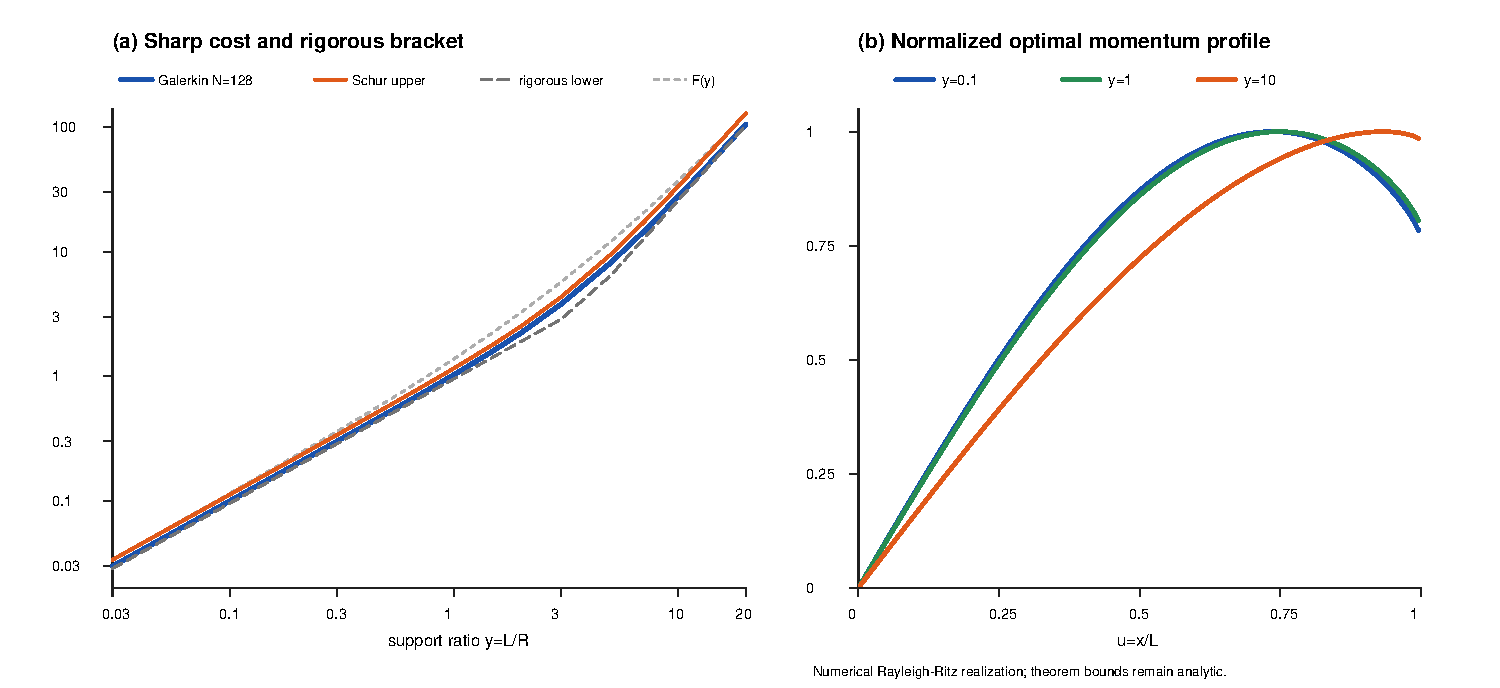
\includegraphics[width=\textwidth]{figures/observer_cost_spectrum.pdf}
 \caption{Numerical realization of the exact compact-kernel theorem.
 Panel (a) compares the $128$-cell Galerkin estimate with the rigorous
 analytic lower bound, the exact-kernel row-Schur upper bound, and the simpler
 closed-form upper bound $F(y)$.  Panel (b) shows the positive top
 eigenfunction, normalized by its maximum, at three support ratios.}
 \label{fig:cost-spectrum}
\end{figure}

Combining \cref{eq:diamond-error,eq:causal-support,eq:sharp-cost} gives the
operational form.

\begin{corollary}[Causal source-cylinder envelope]
\label{cor:source-bound}
If the source in \cref{eq:interaction} is supported in $r\leq a<R$ for a
static-time interval of length $T$, set
\begin{equation}
 y=\operatorname{arctanh}(a/R)+T/R.
\end{equation}
Then
\begin{equation}
 \log\frac{1}{2\eobs}
 \leq \EK R C_{\rm opt}(y)
 =2\EK R y\Lambda(y/2)
 \leq\EK R F(y).
 \label{eq:source-bound}
\end{equation}
The first coefficient is sharp for the relaxed problem in which only the final
Cauchy support $L$ is fixed.  For a cylinder with smaller spatial radius
$\ell=L-T$, the bound remains valid, but reachability of its top eigenfunction
is not asserted.
Exact complete dephasing at finite $a$, $T$, and $R$ requires $\EK=\infty$.
\end{corollary}

\begin{remark}
The final statement is a no-go only for exact complete dephasing in the frozen
local scalar model.  It is not a universal energy cost for quantum
measurement, and it does not price the external device used to realize $J$.
\end{remark}

\section{Finite-pointer entropy and observer-code accuracy}
\label{sec:finite-pointer}

We now compose the sharp binary covariance theorem with the exact
finite-pointer channel.  The composition uses no new spectral estimate.  Its
input is the pairwise form bound; its additional ingredients are the weighted
variance identity and convexity.

Define the ideal classical pointer purity and its second R\'enyi entropy by
\begin{equation}
 \Pcl:=\sum_iw_i^2,
 \qquad H_2(w):=-\log\Pcl.
 \label{eq:classical-pointer-purity}
\end{equation}

\begin{theorem}[Finite-pointer energy--support--entropy bound]
\label{thm:finite-pointer-renyi}
Let $p_i$ be Dirichlet half-line momentum data supported in $[0,L]$, with
$w_i\geq0$ and $\sum_iw_i=1$.  Set
\begin{equation}
 \bar p=\sum_iw_ip_i,
 \qquad
 \Ebar=\frac12\sum_iw_i\norm{p_i-\bar p}^2.
 \label{eq:half-line-centered-energy}
\end{equation}
For the exact thermal channel in \cref{eq:dephasing-channel},
\begin{equation}
 \boxed{
 \Tr\rho_P^2\geq\Pcl+(1-\Pcl)
 \exp\!\left[-\frac{\mathcal C_\beta(L)\Ebar}{1-\Pcl}\right]}
 \label{eq:finite-pointer-purity-bound}
\end{equation}
when $\Pcl<1$, with the continuous value one when $\Pcl=1$.  Consequently,
\begin{align}
 S_2(\rho_P)
 &\leq-\log\left\{\Pcl+(1-\Pcl)
 \exp\!\left[-\frac{\mathcal C_\beta(L)\Ebar}{1-\Pcl}\right]\right\}
 \label{eq:finite-pointer-entropy-bound}\\
 &\leq\min\{H_2(w),\mathcal C_\beta(L)\Ebar\}.
 \label{eq:simple-entropy-bound}
\end{align}
The first inequality is saturated for equal binary weights and opposite
top-eigenfunction profiles.  Global sharpness for arbitrary pointer dimension
is not asserted.
\end{theorem}

\begin{proof}
Write $d_{ij}=p_i-p_j$ and $x_{ij}=2\Gamma_{ij}$.  By
\cref{eq:pairwise-dephasing,eq:general-cost-definition},
\begin{equation}
 x_{ij}=\frac12\ip{d_{ij}}{B_{\beta,L}d_{ij}}
 \leq\frac{\mathcal C_\beta(L)}4\norm{d_{ij}}^2.
 \label{eq:pairwise-exponent-bound}
\end{equation}
The weighted variance identity gives
\begin{equation}
 \sum_{i,j}w_iw_j\norm{p_i-p_j}^2=4\Ebar,
 \label{eq:pairwise-variance-identity}
\end{equation}
and hence
\begin{equation}
 \sum_{i,j}w_iw_jx_{ij}\leq\mathcal C_\beta(L)\Ebar.
 \label{eq:average-exponent-bound}
\end{equation}
The terms $i=j$ have $x_{ii}=0$ and total weight $\Pcl$.  Normalize the
remaining weights by $1-\Pcl$ and apply Jensen's inequality to $e^{-x}$ in
\cref{eq:finite-pointer-purity}; this proves
\cref{eq:finite-pointer-purity-bound}.  The first simple bound follows because
the right side is at least $\Pcl$.  For $z\geq0$, convexity also gives
\begin{equation}
 \Pcl+(1-\Pcl)e^{-z/(1-\Pcl)}\geq e^{-z}.
\end{equation}
Taking $z=\mathcal C_\beta(L)\Ebar$ proves the second bound in
\cref{eq:simple-entropy-bound}.

For two equal weights and $p_\pm=\pm p$, the off-diagonal exponents coincide.
If $p$ is the top eigenfunction of $B_{\beta,L}$, both the form bound and
Jensen's inequality are equalities.  For more pointer states, equality would
require all nonzero differences to lie in the simple top eigenspace and to
have equal exponent.  We do not claim that those conditions can be met.
\end{proof}

The same argument works in the full static-patch phase space because the
energy is a Hilbert norm and \cref{thm:main} bounds the thermal form of every
difference datum.

\begin{corollary}[Conformal de Sitter finite-pointer bound]
\label{cor:de-sitter-finite-pointer}
Let every conditional angular and canonical datum be supported in $[0,yR]$,
and define $\Ebar$ by centering in the full energy norm as in
\cref{eq:centered-field-energy}.  Then
\begin{align}
 \Tr\rho_P^2
 &\geq\Pcl+(1-\Pcl)
 \exp\!\left[-\frac{R C_{\rm opt}(y)\Ebar}{1-\Pcl}\right],
 \label{eq:de-sitter-pointer-purity}\\
 S_2(\rho_P)&\leq\min\{H_2(w),R C_{\rm opt}(y)\Ebar\}.
 \label{eq:de-sitter-pointer-entropy}
\end{align}
The coefficient $C_{\rm opt}(y)=2y\Lambda(y/2)$ is exact.  Binary saturation
uses the unique s-wave momentum optimizer of \cref{thm:main}.
\end{corollary}

\subsection{Insertion into the observer code}

The field record provides a purification of the physical pointer state:
\begin{equation}
 \ket\omega=\sum_i\sqrt{w_i}\ket{i}_{\rm Ob}\ket{e_i}_{\rm Ob'},
 \qquad \ip{e_j}{e_i}=G_{ij}.
 \label{eq:physical-record-state}
\end{equation}
The two reductions of this pure state have identical nonzero spectra, so
\begin{equation}
 e^{-S_2(\omega_{\rm Ob'})}
 =\Tr\omega_{\rm Ob'}^2
 =\Tr\rho_P^2.
 \label{eq:physical-purity-identification}
\end{equation}
This is the entropy parameter appearing in the simple random-code calculation
of Harlow, Usatyuk, and Zhao~\cite{HarlowUsatyukZhao2025}.

\begin{proposition}[Physical floor in the simple observer code]
\label{prop:harlow-floor}
Let $D$ be the dimension of their Haar-random orthogonal encoding matrix, and
let $\ket\phi$, $\ket\psi$ be orthogonal CRT-real matter states.  Replacing
the ideal record by \cref{eq:physical-record-state}, their exact second-moment
formula gives
\begin{equation}
 \mathbb E_O\abs{\bra\phi\widehat V^\dagger\widehat V\ket\psi}^2
 =\frac{D}{D+2}\Tr\rho_P^2.
 \label{eq:harlow-exact-purity}
\end{equation}
Consequently, for the de Sitter model,
\begin{equation}
 \mathbb E_O\abs{\bra\phi\widehat V^\dagger\widehat V\ket\psi}^2
 \geq\frac{D}{D+2}\left\{\Pcl+(1-\Pcl)
 e^{-R C_{\rm opt}(y)\Ebar/(1-\Pcl)}\right\}.
 \label{eq:harlow-physical-floor}
\end{equation}
\end{proposition}

\begin{proof}
Equation~(4.2) of \cite{HarlowUsatyukZhao2025} contains the observer terms
$e^{-S_2(\omega_{\rm Ob'})}$ and
$\Tr(\omega_{\rm Ob}\omega_{\rm Ob}^{T})$ together with two matter overlaps.
For the stated orthogonal CRT-real pair, both overlaps vanish, leaving
\cref{eq:harlow-exact-purity}.  Apply
\cref{eq:physical-purity-identification,eq:de-sitter-pointer-purity}.
\end{proof}

The proposition closes a specific gap: the entropy suppressing the simple
code fluctuation is now generated by a localized field record with an exact
energy--support bound.  Its scope is narrower than a gravitational observer
theorem.  The system called ${\rm Ob'}$ in
\cref{eq:physical-record-state} is the purified nonideal record, and
\cref{eq:harlow-physical-floor} is a Haar-ensemble mean-square statement for
one orthogonal pair.  It is not a deterministic lower bound for every fixed
encoding map.  Nor does it include an autonomous observer, actuator work, or
gravitational evolution.

\section{Optimal profiles and smooth source realization}
\label{sec:construction}

\subsection{Explicit trial profiles}

The exact optimizer in \cref{thm:main} is the top eigenfunction of
$\mathcal K_{y/2}$.  Two elementary profiles give the explicit lower bounds in
\cref{eq:global-explicit-bracket} and make both asymptotic regimes concrete.
For the vacuum-controlled regime, set $L=yR$, choose $q=0$, and use
\begin{equation}
 p_L(x)=\sqrt{\frac{3}{L^3}}\,x\,\mathbf1_{(0,L)}(x).
 \label{eq:linear-profile}
\end{equation}
The vacuum part of the thermal form is
\begin{align}
 \ip{p_L}{h_0^{-1}p_L}
 &=\frac{3}{\pi L^3}
 \int_0^L\!\int_0^L xy
 \log\frac{x+y}{\abs{x-y}}\dd x\dd y \notag\\
 &=\frac{3L}{2\pi}.
 \label{eq:linear-profile-covariance}
\end{align}
For the second equality, scale $x=Lu$, $y=Lv$, split the unit square across
the diagonal, and use
\begin{equation}
 \int_0^1 t\log\frac{1+t}{1-t}\dd t=1.
\end{equation}
Since $\coth(\beta h_0/2)\geq1$, the full thermal dephasing exponent is at
least the value in \cref{eq:linear-profile-covariance}.  On the other hand,
$\EK=1/2$ for the normalized datum.  Thus
$\Gamma/(\EK R)\geq3L/(\pi R)=3y/\pi$.

For the thermal regime, use instead the normalized first eigenfunction of the
Dirichlet--Neumann Green operator,
\begin{equation}
 p_L^{\rm th}(x)=\sqrt{\frac2L}\sin\frac{\pi x}{2L}
 \mathbf1_{(0,L)}(x).
 \label{eq:thermal-profile}
\end{equation}
Since $\coth z\geq z^{-1}$ and
$\ip{p_L^{\rm th}}{h_0^{-2}p_L^{\rm th}}=4L^2/\pi^2$, this datum gives
\begin{equation}
 \frac{\Gamma}{\EK R}\geq\frac{8y^2}{\pi^3}.
\end{equation}
The first profile and the vacuum Schur bound also show
\begin{equation}
 \frac{3}{\pi}
 \leq\liminf_{y\downarrow0}\frac{C_{\rm opt}(y)}y
 \leq\limsup_{y\downarrow0}\frac{C_{\rm opt}(y)}y
 \leq\frac{4\operatorname{arsinh}(1)}\pi.
 \label{eq:small-support-gap}
\end{equation}
The ratio of the analytic upper and lower linear coefficients is
$4\operatorname{arsinh}(1)/3\simeq1.17516$.

For a target exponent $\Gamma_\star$, scaling
\cref{eq:linear-profile} by an amplitude $A$ yields the sufficient energy
bound
\begin{equation}
 \EK\leq\frac{\pi\Gamma_\star}{3L}.
 \label{eq:constructive-energy}
\end{equation}
This is an upper bound on the energy needed by this simple family.  The sharp
half-line momentum infimum at inverse temperature $\beta$ is instead
$\Gamma_\star/\mathcal C_\beta(L)
=\Gamma_\star/[2L\Lambda(\pi L/\beta)]$.  At the de Sitter temperature this
is $\Gamma_\star/[R C_{\rm opt}(L/R)]$.

\subsection{Smooth compact sources}

The hard endpoint in \cref{eq:linear-profile} is useful for exact constants
but is not a smooth source.  We now show that it is a legitimate limiting
profile and that every strict window persists.

\begin{lemma}[Smooth density closure]
\label{lem:smooth-density}
Fix an optical source radius $\ell>0$ and a normalized
$p\in L^2(0,\ell)$.  There are normalized
$p_n\in C_c^\infty([0,\ell))$, regular at the origin, such that
\begin{equation}
 p_n\longrightarrow p
 \quad\hbox{in }L^2(\R_+).
 \label{eq:smooth-convergence}
\end{equation}
Their thermal dephasing forms converge, and their cumulative energy measures
converge uniformly.
\end{lemma}

\begin{proof}
Density of smooth functions supported strictly inside $(0,\ell)$ gives
\cref{eq:smooth-convergence}; such functions are automatically regular radial
data at the origin.  On data supported in $[0,\ell]$,
\begin{equation}
 P_\ell h_0^{-1}\coth(\beta h_0/2)P_\ell
 \leq P_\ell h_0^{-1}P_\ell
 +\frac2\beta P_\ell h_0^{-2}P_\ell
 \label{eq:thermal-compressed-bound}
\end{equation}
as quadratic forms.  The right side is bounded by
\cref{lem:compressed-inverses}; hence the covariance is continuous under
$L^2$ convergence.  Finally,
\begin{equation}
 \sup_{0\leq x\leq\ell}
 \left|\int_0^x(p_n^2-p^2)\dd s\right|
 \leq\norm{p_n-p}_2(\norm{p_n}_2+\norm p_2),
 \label{eq:mass-uniform-convergence}
\end{equation}
which proves uniform convergence of cumulative energy.
\end{proof}

It remains to produce a supported final datum by a smooth spacetime source.
This also proves sharpness over sources when the source ball approaches the
declared final-support ball; it does not prove exact controllability from a
strictly smaller cylinder of optical radius $L-T$.  Let
$\phi_{\rm free,n}$ be the homogeneous solution with final data
$(q,p)=(0,p_n)$.  Choose a smooth time cutoff $\eta_n$ that vanishes before
the protocol, equals one near the final slice, and changes over a time shorter
than the optical gap between $\supp p_n$ and $\ell$.  If $\mathcal P$ is the
conformal wave operator, set
\begin{equation}
 J_n=\mathcal P(\eta_n\phi_{\rm free,n}).
 \label{eq:smooth-source}
\end{equation}
The retarded solution sourced by $J_n$ is
$\eta_n\phi_{\rm free,n}$.  It therefore has exactly the desired final data.
Finite propagation keeps $J_n$ inside the declared optical worldtube.  This
construction proves smooth source existence, but it does not bound the stress
of an autonomous mechanism that generates the prescribed $J_n$.

For a finite pointer, apply this construction to each conditional datum
separately and take a common cutoff interval and worldtube.  Because only
finitely many branches are present, the approximations can be chosen so that
all branch energies and all pairwise thermal forms converge simultaneously.
The resulting diagonal controlled source therefore realizes the Schur
channel used in \cref{thm:finite-pointer-renyi}.  This observation establishes
finite-pointer source closure; it does not add a general-$d$ saturation claim.

\section{Relation to prior bounds and detector work}
\label{sec:comparison}

\subsection{Bekenstein entropy is a different quadratic form}

For a Klein--Gordon wave packet localized in a spatial region of half-width
$a$, Hollands, Longo, and Morsella prove the Bekenstein-type inequality
\begin{equation}
 S(\Phi\mid B)\leq2\pi a E,
 \label{eq:bekenstein-bound}
\end{equation}
where $S(\Phi\mid B)$ is the entropy quadratic form of the local standard
subspace~\cite{HollandsLongoMorsella2026}.  At second quantization this is the
relative entropy of the corresponding coherent excitation.  This powerful
result is directly adjacent to \cref{thm:thermal-half-line}, but it controls a
different functional.

We make the distinction explicit in the simplest common setting.  Consider
the massless conformal vacuum in four-dimensional Minkowski space, restrict to
radial $q=0$ data in a ball of radius $a$, and normalize $\norm{p}_2=1$.  The
conformal-ball modular Hamiltonian and the half-line dephasing kernel give
\begin{align}
 S_B[p]
 &=\frac{\pi}{2a}\int_0^a(a^2-x^2)p(x)^2\dd x,
 \label{eq:SB-form}\\
 \Gamma_0[p]
 &=\ip p{h_0^{-1}p}
 =\frac1\pi\int_0^a\!\int_0^a p(x)p(y)
 \log\frac{x+y}{\abs{x-y}}\dd x\dd y.
 \label{eq:Gamma0-form}
\end{align}

\begin{proposition}[Quadratic-form separation]
\label{prop:bekenstein-separation}
At fixed $a$, there is no finite constant $c$ such that
$\Gamma_0[p]\leq cS_B[p]$ for all smooth normalized radial momenta, and no
finite constant $c'$ such that $S_B[p]\leq c'\Gamma_0[p]$ for all such data.
\end{proposition}

\begin{proof}
Let $f\in C_c^\infty(0,1)$ be positive and normalized in $L^2(0,1)$.  For a
packet in a boundary layer, set
\begin{equation}
 p_\delta^{\rm wall}(x)
 =\delta^{-1/2}f\!\left(\frac{a-x}{\delta}\right).
\end{equation}
Substitution in \cref{eq:SB-form} gives
\begin{equation}
 S_B[p_\delta^{\rm wall}]
 =\pi\delta\int_0^1u f(u)^2\dd u+O(\delta^2).
 \label{eq:SB-wall}
\end{equation}
For the logarithmic kernel, scaling both variables gives
\begin{equation}
 \Gamma_0[p_\delta^{\rm wall}]
 =\frac{\delta}{\pi}\left(\int_0^1f(u)\dd u\right)^2
 \log\frac1\delta+O(\delta).
 \label{eq:Gamma-wall}
\end{equation}
Thus $\Gamma_0/S_B\to\infty$.

For a packet near the center, set
\begin{equation}
 p_\delta^{\rm ctr}(x)=\delta^{-1/2}f(x/\delta).
\end{equation}
Then
\begin{equation}
 S_B[p_\delta^{\rm ctr}]=\frac{\pi a}{2}+O(\delta^2),
 \qquad
 \Gamma_0[p_\delta^{\rm ctr}]=O(\delta),
 \label{eq:center-asymptotics}
\end{equation}
because the logarithmic kernel becomes scale invariant after
$x=\delta u$, $y=\delta v$, while the two integration measures leave one
factor of $\delta$.  Hence $S_B/\Gamma_0\to\infty$.
\end{proof}

The separation has a simple physical meaning.  The Bekenstein entropy is a
local modular-information functional whose conformal weight vanishes at the
ball boundary.  The zero-temperature dephasing exponent is a global
one-particle norm, equivalently an entangling-particle count for the exact
detector model.  At finite temperature, the factor $\coth(\beta h/2)$ enhances
infrared fluctuations further.  Thermal dephasing can increase even while the
distinguishability of two displaced thermal states decreases.  The two notions
of information should not be identified.

\subsection{Relation to DSW and exact detector work}

DSW decoherence describes the loss of coherence of superposed charges or
masses near Killing horizons through soft field modes
\cite{DSW2023,DSW2025}.  Gralla and Wei gave a general horizon formulation and
precise rates in electromagnetic and Klein--Gordon analogues
\cite{GrallaWei2024}; Li evaluated the local scalar, electromagnetic, and
gravitational cases in de Sitter~\cite{Li2025}.  These works establish the
physical importance of the low-frequency KMS sector that appears in
\cref{eq:gamma-sector}.

Our setup differs in its question.  We do not derive a new horizon decoherence
rate.  We start from the exact pointer channel and maximize its dephasing
functional subject to finite final support and post-switch field energy.  The
result is consequently a constraint on a local implementation, not a claim
that horizon modes require a large Killing energy.  Indeed, sufficiently soft
horizon radiation can carry negligible Killing energy when its support and
duration are allowed to grow.  In \cref{eq:source-bound}, that escape route is
visible in the growth of $C_{\rm opt}$ with $L=\ell+T$.

Barcellos and Landulfo already separate field background energy, individual
switching work, and communication work for the exact gapless-detector channel
\cite{BarcellosLandulfo2021}.  We use their same exact channel class.  The new
step is to eliminate the source amplitude, identify the exact compact KMS
kernel, and solve the full final-support optimization.  We therefore make no
novelty claim for Magnus termination, the KMS characteristic function, the
coherent stress identity, or switching-energy accounting.

Related Unruh--DeWitt-gate work represents relativistic communication
channels as bosonic dephasing channels whose parameters depend on coupling,
smearing, and switching data~\cite{AsplingLawler2023}.  That work concerns
channel structure and capacity rather than the post-switch field-energy and
final-support variational problem posed here.

Likewise, spectral extremization of Riesz-potential operators is not new
\cite{RuzhanskySuragan2016}, and largest-eigenvalue questions for logarithmic
potentials have an established literature~\cite{AnoopJohnson2025,
JohnsonVerma2026}.  There are two exact relationships that sharpen this
comparison.  First, let $\widetilde p$ be the odd extension of $p$ from
$(0,1)$ to $(-1,1)$.  The zero-temperature operator is precisely the odd
sector of the finite-interval logarithmic convolution:
\begin{equation}
 \frac1\pi\int_{-1}^{1}\log\frac1{\abs{u-v}}\,
 \widetilde p(v)\dd v
 =\int_0^1 k_0(u,v)p(v)\dd v,
 \qquad 0<u<1.
 \label{eq:odd-log-convolution}
\end{equation}
Polosin studies high-index eigenvalue and eigenfunction asymptotics of that
convolution in its even and odd sectors~\cite{Polosin2022}.  Thus the vacuum
convolution problem itself is not new; that work does not give the thermal
principal-support law or the uniform temperature remainders used here.

Second, for $\tau>0$, set $r=e^{-2\tau u}$ and
$s=e^{-2\tau v}$.  Directly,
\begin{equation}
 k_\tau(u,v)=\frac1\pi\log\frac{1-rs}{\abs{r-s}}.
 \label{eq:hyperbolic-cross-ratio}
\end{equation}
The ratio on the right is the inverse pseudo-hyperbolic distance between two
points on a diameter of the Poincare disk.  The change of variables turns
$L^2(0,1)$ into
$L^2((e^{-2\tau},1),\dd r/(2\tau r))$.  Hence our operator is a weighted
one-dimensional geodesic compression of the hyperbolic logarithmic Green
kernel, not the two-dimensional hyperbolic-area operator studied in
\cite{JohnsonVerma2026}.

At the quadratic-form level, odd extension also writes the localized operator
$B_{\beta,L}$ as a finite-interval Wiener--Hopf term minus its Hankel image,
generated by the singular even multiplier
$\abs{k}^{-1}\coth(\beta\abs{k}/2)$.  The zero-frequency singularities of the
two image terms cancel in their Dirichlet difference.  This places the
operator near work on singular truncated Wiener--Hopf inverses and
determinants~\cite{Widom2006,Kozlowski2008}, although those results concern
different spectral quantities and symbol hypotheses.

Thus the claim here is not a first eigenvalue theorem for an unspecified
positive compact kernel.  It is the identification of the exact reflected
thermal operator governing this local pointer channel, proof that it controls
the complete canonical and angular phase space, and extraction of uniform
support laws with explicit constants.  The comparisons above do not by
themselves establish priority; they make the remaining operator-theory
novelty question precise.

\section{Discussion and claim boundary}
\label{sec:discussion}

The result has two layers.  The analytic engine is the exact localization
coefficient for the thermal inverse Hamiltonian.  The physical composition is
the finite-pointer purity bound and its insertion into a simple observer code.
Together they say that a field record of large second R\'enyi entropy cannot be
produced with simultaneously fixed support and bounded post-switch scalar
energy in this model.  The statement is quantitative and nonperturbative in
the source amplitude.

Compact final support is the decisive hypothesis.  Without it, arbitrarily
soft thermal modes prevent an energy norm from controlling the dephasing
form.  With it, the compressed inverse Hamiltonian is bounded.  At arbitrary
inverse temperature its norm is governed by
$\mathcal K_{\pi L/\beta}$; in conformal de Sitter, angular resolvent order and
a separate field-coordinate estimate show that the same s-wave momentum mode
controls the complete canonical and angular phase space.  The
temperature--curvature relation enters only in this all-sector reduction.

\subsection{What is established}

The exact statements are:
\begin{enumerate}[leftmargin=*,itemsep=2pt]
 \item a controlled-source realization of the finite-pointer Schur channel,
 with pairwise exponents fixed by conditional field differences;
 \item the arbitrary-$\beta$ coefficient
 $\mathcal C_\beta(L)=2L\Lambda(\pi L/\beta)$, its simple top mode, global
 bracket, and uniform support asymptotics;
 \item the conformal de Sitter reduction of every angular and canonical sector
 to that unique s-wave momentum optimizer;
 \item the purity and R\'enyi bounds
 \cref{eq:finite-pointer-purity-bound,eq:simple-entropy-bound}, with exact
 saturation for the symmetric binary top-mode record;
 \item the physical-purity insertion
 \cref{eq:harlow-physical-floor} into the Harlow--Usatyuk--Zhao simple random
 code for an orthogonal CRT-real matter pair; and
 \item the branchwise final-slice constraint estimate
 \cref{eq:branchwise-gravity-renyi} for spherical $q_i=0$ records.
\end{enumerate}

The finite-pointer theorem is not claimed to be globally sharp at arbitrary
dimension.  Simultaneous equality would require every nonzero pairwise
difference to align with one simple top eigenspace and all off-diagonal
exponents to coincide.  The binary construction meets those conditions; a
generic larger alphabet does not.

Sharpness of the operator coefficient refers to final Cauchy data supported
in $[0,L]$.  For a source cylinder with optical radius $\ell<L$ and duration
$T=L-\ell$, finite propagation proves the same upper bound but not
near-controllability of its top eigenfunction.  Smooth compact sources do
approach every final-support Rayleigh quotient when their worldtube approaches
the declared final-support ball.

\subsection{Observer-code interpretation}

The code insertion supplies a concrete bridge that the earlier binary
diamond-error comparison did not.  The conditional field record purifies the
physical pointer state, so its record-system purity is exactly
$\Tr\rho_P^2$.  For the specified orthogonal CRT-real pair, this is precisely
the observer factor left in the Haar second moment of
\cite{HarlowUsatyukZhao2025}.  The field theorem therefore converts a
localization and energy budget into a lower floor on that ensemble-averaged
squared inner-product fluctuation.

This remains narrower than a gravitational observer theorem.  The result
does not bound the error of every fixed encoding map, establish a
high-probability statement, or control all matter pairs at once.  It also
does not identify the scalar energy with a total observer mass.  Harlow's
Hartle--Hawking extension separately argues that the formal
$S_{\rm Ob}\to\infty$ limit likely requires an infinitely heavy
observer~\cite{Harlow2026Observers}.  Our result realizes a related
energy--entropy obstruction in one field-record sector; it is not a
derivation of that broader claim.

The field-energy quantity is the post-switch scalar Killing energy of the
coherent conditional displacements.  It excludes the work, clock, battery,
trap, material support, and stress needed to implement the prescribed
sources.  The shared finite pointer is a gapless-detector idealization rather
than an autonomous relativistic probe field.  Accordingly, the theorem is not
a universal measurement-energy principle.

The gravity corollary is likewise deliberately branchwise and kinematical.
Each conditional spherical datum is placed on its own exact
Einstein--scalar final slice and must satisfy the local budget separately.
The quantum channel is still evaluated on the unperturbed de Sitter
background.  We do not derive a common branch-dependent quantum evolution,
include actuator stress, or prove global closeness to pure de Sitter; the
compact mass shifts the cosmological horizon.

\subsection{Novelty boundary}

Exact gapless-detector channels, their thermal damping factors, and their
field-energy accounting are prior art.  Positive compact kernels, simple top
eigenvalues, logarithmic-potential operators, and Riesz-potential
variational principles are also established mathematics.  The candidate
contribution is their specific composition here: the reflected thermal
operator selected by final support, its exact all-sector de Sitter norm, the
finite-pointer R\'enyi resource bound, and the resulting observer-code
mean-square floor.

The localized Klein--Gordon entropy comparison in \cref{sec:comparison}
shows that this purity functional is not a repackaging of the recent
Bekenstein bound.  It is not a second headline.  Independent review in
relativistic detector theory, integral-operator or fractional-Sobolev theory,
and quantum gravity remains the binding publication gate.

\subsection{Extensions}

A first physical strengthening would replace the Haar mean-square statement
by a concentration or high-probability theorem over the code ensemble.  That
requires controlling correlations among matter pairs and is not supplied by
the present second moment.  A second would replace the prescribed pointer by
a localized relativistic probe field, following the detector-from-field
framework of \cite{PercheEtAl2024}, while retaining the localization theorem
and accounting for the probe stress tensor.

The direct mathematical extension is the true fixed-source-cylinder
optimization.  It requires either a near-controllability theorem for sources
in a prescribed smaller worldtube or a source-to-final-data singular-value
problem replacing $\Lambda$.  A broader geometric extension would identify
conditions under which localized norms of
$h^{-1}\coth(\beta h/2)$ admit comparable sharp constants on other static
spacetimes.

\subsection{Reproducibility}

From the repository root, the analytic records, independent finite-pointer
replay, numerical illustration, and focused checks are reproduced by
\begin{verbatim}
PYTHONPATH=. python experiments/local_scalar_observer_cost_audit.py
PYTHONPATH=. python experiments/local_scalar_observer_spectrum.py
PYTHONPATH=. python experiments/finite_pointer_observer_audit.py
PYTHONPATH=. python experiments/finite_pointer_observer_clean_room_check.py
PYTHONPATH=. python -m pytest -q \
  tests/test_local_scalar_observer_cost.py \
  tests/test_local_scalar_observer_manuscript.py \
  tests/test_local_scalar_observer_spectrum.py \
  tests/test_finite_pointer_observer.py
\end{verbatim}
The frozen records check formulas, source hashes, numerical convergence, and
artifact provenance.  They do not replace the analytic proofs or certify
literature novelty.

\appendix
\section{Final-slice Einstein--scalar application}
\label{sec:gravity}

This appendix is not part of the paper's headline theorem.  The all-angular
de Sitter result does not require spherical symmetry.  We now restrict
to the s-wave and to a final slice on which the radial field coordinate
vanishes.  This subclass is useful because its momentum density vanishes and
its energy measure has a direct constraint interpretation.

Let $u(t,x)$ be the normalized rescaled s-wave.  The physical conformal scalar
is
\begin{equation}
 \phi(t,r)=\frac{u(t,x(r))}{\sqrt{4\pi}\,r}.
 \label{eq:physical-radial-field}
\end{equation}
On a final slice with $u=0$ and $p=\partial_tu$, the physical normal derivative
in the de Sitter geometry is
\begin{equation}
 v(r):=n^a\nabla_a\phi
 =\frac{p(x(r))}{\sqrt{4\pi}\,r\sqrt{N(r)}}.
 \label{eq:normal-derivative}
\end{equation}
For the conformally coupled stress tensor, every improvement term containing
$\phi$ or a spatial derivative of $\phi$ vanishes on this slice.  Directly,
\begin{equation}
 \rho=T_{ab}n^an^b=\frac12v^2,
 \qquad
 j_i=-T_{ab}n^ah^b{}_i=0.
 \label{eq:flux-free-stress}
\end{equation}
Since $\dd r=N\dd x$, \cref{eq:normal-derivative,eq:flux-free-stress} imply
the exact measure identity
\begin{equation}
 4\pi r^2\rho(r)\dd r=\frac12p(x)^2\dd x.
 \label{eq:mass-energy-measure}
\end{equation}

Use the same numerical function $v$ as the scalar normal-momentum datum on a
new spherical initial slice, and consider gravitational data with vanishing
extrinsic curvature,
\begin{equation}
 \dd l^2=\frac{\dd r^2}{f(r)}+r^2\dd\Omega_2^2,
 \qquad K_{ij}=0,
 \qquad
 f(r)=N(r)-\frac{2Gm(r)}{r}.
 \label{eq:constraint-metric}
\end{equation}
The momentum constraint is satisfied by \cref{eq:flux-free-stress}.  The
Hamiltonian constraint with cosmological radius $R$ is solved by
\begin{equation}
 m'(r)=4\pi r^2\rho(r),
 \qquad m(0)=0.
 \label{eq:mass-constraint}
\end{equation}
Absorbing the Bunch--Davies vacuum expectation into the background
cosmological constant, the coherent excess stress in
\cref{eq:energy-stress} supplies precisely the classical source above.
Although $K_{ij}=0$, the nonzero scalar normal momentum means that the full
Einstein--scalar data are not invariant under time reflection.
Equation~\eqref{eq:mass-energy-measure} then gives
\begin{equation}
 m(b)=\EK
 \label{eq:mass-equals-energy}
\end{equation}
for any areal radius $b$ outside the field support.

Define the dimensionless radial constraint ratio
\begin{equation}
 Q(r)=\frac{2Gm(r)}{rN(r)}.
 \label{eq:constraint-ratio}
\end{equation}
For a comparison ball $0<r\leq b<R$, set
\begin{equation}
 Q_b:=\sup_{0<r\leq b}Q(r).
\end{equation}
If $Q_b\leq\delta<1$, then throughout that ball
\begin{equation}
 f(r)\geq N(r)(1-\delta)>0,
 \qquad
 0\leq\frac{g_{rr}}{g_{rr}^{\rm dS}}-1
 \leq\frac{\delta}{1-\delta}.
 \label{eq:metric-control}
\end{equation}

\begin{corollary}[Necessary final-slice constraint cost]
\label{cor:gravity-cost}
Let the hypotheses of \cref{cor:source-bound} hold and suppose the source is
engineered to finish with spherical $q=0$ data.  Set
\begin{equation}
 b=R\tanh(L/R),
 \qquad L=R\operatorname{arctanh}(a/R)+T.
\end{equation}
Then
\begin{equation}
 Q_b\geq Q(b)
 \geq
 \frac{2G}{bN(b)R C_{\rm opt}(L/R)}
 \log\frac{1}{2\eobs}.
 \label{eq:gravity-lower-bound}
\end{equation}
Equivalently, a local budget $Q_b\leq\delta<1$ implies
\begin{equation}
 \eobs\geq\frac12\exp\left[
 -\frac{\delta\,bN(b)R}{2G}C_{\rm opt}(L/R)
 \right].
 \label{eq:gravity-error-floor}
\end{equation}
\end{corollary}

\begin{proof}
Outside the support, \cref{eq:mass-equals-energy} gives
$Q(b)=2G\EK/[bN(b)]$.  Apply the sharp energy lower bound in
\cref{cor:source-bound}; solving the same inequality in the other direction
gives \cref{eq:gravity-error-floor}.
\end{proof}

The compact mass shifts the cosmological horizon relative to the pure de
Sitter value $R$.  Accordingly, $Q_b$ is a local comparison norm on the ball
containing the final datum; no global smallness claim relative to the
unperturbed lapse is intended.

\subsection{An explicit local weak-constraint window}

For the source optical radius
$\ell=R\operatorname{arctanh}(a/R)$, take the ideal profile
\begin{equation}
 q=0,
 \qquad
 p(x)=A\sqrt{\frac{3}{\ell^3}}x\mathbf1_{(0,\ell)}(x).
 \label{eq:gravity-profile}
\end{equation}
Its cumulative mass is
\begin{equation}
 m(x)=\EK\left(\frac{x}{\ell}\right)^3.
 \label{eq:cumulative-mass}
\end{equation}
Inside the support, the function
\begin{equation}
 \frac{\operatorname{arctanh}(r/R)^3}{r[1-r^2/R^2]}
 \label{eq:q-monotone-function}
\end{equation}
is strictly increasing on $(0,a]$.  One way to see this is to factor it as
$(x/r)(x^2/N)$; both factors increase with $r$.  Hence the wall value controls
the complete profile.  Combining \cref{eq:constructive-energy} with the wall
constraint gives the sufficient estimate
\begin{equation}
 Q_a
 \leq\frac{2\pi G\Gamma_\star}
 {3\ell\,a[1-a^2/R^2]}.
 \label{eq:constructive-gravity}
\end{equation}

For illustration, set
\begin{equation}
 \eobs=10^{-6},\quad
 a/R=0.2,\quad T/R=0.1,\quad
 G/R^2=10^{-6},\quad \delta=0.25.
\end{equation}
The universal theorem requires
\begin{equation}
 C_{\rm opt}(L/R)\leq0.340766570374,
 \qquad \EK R\geq38.5083647231,
 \qquad Q(b)\geq2.86896268303\times10^{-4},
\end{equation}
whereas the constructive family has
\begin{equation}
 \EK R\leq67.7824380936,
 \qquad Q_a\leq7.06067063475\times10^{-4}.
\end{equation}
Thus the fixed numerical point has a nonempty local weak-constraint window.  By
\cref{lem:smooth-density}, smooth compact profiles preserve this strict
margin.

The construction closes only the final Hamiltonian and momentum constraints.
It does not specify the lapse, evolve the Einstein--scalar system, include the
source actuator during switching, or recompute the quantum channel in the
perturbed geometry.


\begingroup
\small
\let\originalthebibliography\thebibliography
\renewcommand{\thebibliography}[1]{%
  \originalthebibliography{#1}%
  \setlength{\itemsep}{0pt}%
  \setlength{\parskip}{0pt}%
}
\bibliographystyle{unsrt}
\bibliography{references}
\endgroup

\end{document}
